% Short version for DASA'26 (at most 5 pages; required sections: Introduction,
% Methods, Results and Discussion, Conclusion, Acknowledgments, References).
% The full version is main.tex. Both use generated/ and figures/ from make_figures.py.
\documentclass[conference]{IEEEtran}
\usepackage[utf8]{inputenc}
\usepackage{amsmath}
\usepackage{graphicx}
\usepackage{booktabs}
\usepackage{array}
\usepackage{url}
\usepackage{xurl}
\usepackage{xcolor}
\usepackage{siunitx}
\usepackage{tikz}
\usetikzlibrary{positioning,arrows.meta,shapes.geometric,shadows,calc}
\usepackage[hidelinks]{hyperref}
\sisetup{group-separator={,},group-minimum-digits=4}

\newcommand{\CapA}{223}
\newcommand{\CapCOne}{7,500}


\begin{document}

\title{Surviving Result Day: A Measured Decision Guide\\for Building Examination-Result Websites}

\author{\IEEEauthorblockN{Sankalp Pathak and Imran Khan}
\IEEEauthorblockA{Department of Computer Science and Engineering,
Azad Institute of Engineering and Technology, Lucknow, India\\
(affiliated to Dr.~A.~P.~J.~Abdul Kalam Technical University)\\
pathaksankalp04@gmail.com, pe.imran@gmail.com}}

\maketitle

\begin{abstract}
On result day, lakhs of students try to open an examination board's website at
the same moment, and these websites often fail. Boards need evidence to decide
how to build them. We present ResultBench, an open-source testbed that compares
designs of a result website under identical conditions. It runs eleven designs
on the same two processor threads: a website that builds every page from a
database, two mirror copies of it, four variants of a cache in front of the
database, results prepared in advance in an in-memory store or as one file per
student, and virtual waiting rooms in front of these. A
load generator replays a result-day surge of synthetic students who arrive
before and after the announced time, wait a limited time for an answer and
press refresh when it is slow. Every answer is checked against the true
result, so wrong, outdated and missing results are counted alongside speed and
processor use, and every configuration is repeated three times. On one
machine, the database design served only 30.8 percent of students within five
seconds at twice the load it was sized for, while results prepared in advance
served every student at ten times that load, using less than a twelfth of the
processor time per student. No design returned wrong results, a cache helped
only when filled before release, and a waiting room could serve almost every
student, but only after waits of minutes. We turn these measurements into a
decision guide for examination boards.
\end{abstract}


\begin{IEEEkeywords}
examination results, flash crowds, web architecture, waiting rooms, decision guide
\end{IEEEkeywords}

\section{Introduction}

When an Indian examination board declares results, lakhs of students try to
open the result website at the same time~\cite{ht2021ssc}. The release time is
announced in advance, almost every request asks for one roll number, and the
results do not change while students read them. Few web workloads are
simpler, yet result websites keep failing. The chairman of JEE Advanced 2016
described the portal receiving about \num{10000} requests per second against
a server that could hold \num{2000}~\cite{pagalguy2016jee}. On Maharashtra SSC
result day in 2021, schools reported that at least half of their students
could not see results until evening~\cite{ht2021ssc}, and the state's
education minister apologised~\cite{careerindia2021ssc}. Kenya's examination
council reported up to \num{300000} hits per second~\cite{knec2025x}, and in
2025 WAEC in Nigeria withdrew its result checker over \emph{wrong}
results~\cite{icir2025waec}.

A board that wants to avoid this has to decide how to build its website, and
the options are well known: caching or pre-generating
pages~\cite{challenger1999scalable,labrinidis2000webview}, protecting caches
against stampedes~\cite{vattani2015xfetch,nishtala2013memcache}, admission
control~\cite{welsh2001seda,elnikety2004gatekeeper,chen2005news}, and
``virtual waiting rooms'' that queue visitors during surges, sold as
products~\cite{cloudflare2026wr,aws2022vwr} and studied in WebQ, which tells
users of an overloaded server how long to wait and checks with a token that
they did~\cite{doshi2015webq}. What is missing is evidence about which option
works for this workload. Flash-crowd studies characterise crowds and absorb
them with caching~\cite{ari2003flash,jung2002flash,wendell2011going}, but
these crowds are often unforeseen, while a result release is announced. The closest recent studies compare a database-only design with a
Redis cache for university systems under a fixed number of users, one with a
real database~\cite{putranto2026redis} and one with simulated
delays~\cite{tofan2026cacheaside}; neither tests pre-computed results or
waiting rooms, models students who refresh, or checks that the answers are
correct. To our knowledge, no study has compared waiting rooms with other
designs under an announced surge of students who refresh.

This paper gives boards measured evidence for four decisions: which
architecture to use (Q1), whether to put a waiting room in front of it (Q2),
how to keep results correct when they are corrected or released early (Q3),
and how caches and refreshing students change the load (Q4). We contribute
ResultBench, an open-source testbed that runs eleven designs under one
resource budget, replays a result-day surge of students who refresh, and
checks every answer against ground truth; a controlled comparison of the
designs; and a decision guide that turns the measurements into advice
(Table~\ref{tab:guide}).

\section{Methods}
\label{sec:method}

\subsection{Designs}
\label{sec:designs}

Every design answers \texttt{GET /result?roll=$n$} with the same JSON body and
gets the same budget of two CPUs (hardware threads) for answering students
(Fig.~\ref{fig:designs}). Before the announced release time every design
answers ``not released''.
\textbf{A} builds each page from PostgreSQL (a 4-table join).
\textbf{M} splits the budget into two independent copies of A (``mirror
links''); each student picks one at random and, on retry, switches with
probability 0.5.
\textbf{B0} puts a Redis cache in front of A (cache-aside); \textbf{B1} adds
request coalescing, \textbf{B2} probabilistic early
recomputation~\cite{vattani2015xfetch}, and \textbf{B3} fills the cache before
release.
\textbf{C1} pre-computes every result into Redis, and \textbf{C2} writes one
JSON file per student, served by Nginx; both keep an idle back-office
PostgreSQL (0.25 CPU, counted in cost).
\textbf{D} puts a waiting room (0.25 CPU) in front of A, C1 or C2 (we test
D-A and D-C1). It admits
students at 80\% of the backend's capacity, either first come, first served
(FIFO) or by a lottery among early arrivals, as some products
offer~\cite{cloudflare2026queue}. Its ticket is either \emph{naive} (held in
the page and lost when the student presses refresh) or a signed \emph{token}
cookie (kept on refresh). An admitted student may use the backend for
\SI{60}{s}; the waiting room limits neither how many admitted students are
active nor how many requests each sends.

\begin{figure*}[t]
% Read paths of the designs (Section III). Included by sections/designs.tex.
\tikzset{
  box/.style={draw, rounded corners=1.5pt, minimum height=7mm, minimum width=13mm,
              inner sep=2pt, align=center, font=\footnotesize, fill=white},
  stu/.style={box, fill=gray!12},
  app/.style={box, fill=blue!8},
  db/.style={draw, cylinder, shape border rotate=90, aspect=0.22, minimum height=8mm,
             minimum width=14mm, inner sep=1pt, align=center, font=\footnotesize, fill=orange!12},
  kv/.style={db, fill=red!10},
  files/.style={box, fill=green!10, double copy shadow={shadow xshift=1.2pt, shadow yshift=1.2pt}},
  wr/.style={box, fill=yellow!20},
  req/.style={-{Stealth[length=1.8mm]}, semithick},
  pre/.style={-{Stealth[length=1.8mm]}, semithick, dashed, gray!60!black},
  lab/.style={font=\scriptsize, inner sep=1pt, fill=white},
}
\newcommand{\panel}[2]{\begin{minipage}[b]{0.325\textwidth}\centering
  \begin{tikzpicture}[node distance=4mm and 6mm]#2\end{tikzpicture}\par\vspace{2pt}
  {\footnotesize #1}\end{minipage}}
\centering
\panel{(A) Database-backed: every request\\builds the page (+5\,ms CPU)}{%
  \node[stu] (s) {Students};
  \node[app, right=of s] (a) {App};
  \node[db, right=of a] (d) {Postgre-\\SQL};
  \draw[req] (s) -- (a); \draw[req] (a) -- (d);
}\hfill
\panel{(M) Mirrors: two copies of A,\\each with half the CPU}{%
  \node[stu] (s) {Students};
  \node[app, right=of s, yshift=5mm] (a1) {App 1};
  \node[app, right=of s, yshift=-5mm] (a2) {App 2};
  \node[db, right=of a1, minimum height=6.5mm] (d1) {DB 1};
  \node[db, right=of a2, minimum height=6.5mm] (d2) {DB 2};
  \draw[req] (s) -- (a1); \draw[req] (s) -- (a2);
  \draw[req] (a1) -- (d1); \draw[req] (a2) -- (d2);
}\hfill
\panel{(B) Cache-aside: Redis first,\\database only on a miss}{%
  \node[stu] (s) {Students};
  \node[app, right=of s] (a) {App};
  \node[kv, right=of a, yshift=6mm, minimum height=6.5mm] (r) {Redis};
  \node[db, right=of a, yshift=-6mm, minimum height=6.5mm] (d) {Postgre-\\SQL};
  \draw[req] (s) -- (a);
  \draw[req] (a.north east) -- node[lab, above left=0pt] {1: look up} (r.west);
  \draw[req] (a.south east) -- node[lab, below left=0pt] {2: miss} (d.west);
}

\vspace{4mm}
\panel{(C1) Results pre-computed into\\Redis before release}{%
  \node[stu] (s) {Students};
  \node[app, right=of s] (a) {App};
  \node[kv, right=of a] (r) {Redis};
  \node[db, above=5mm of r, minimum height=6.5mm, fill=orange!6] (d) {back office};
  \draw[req] (s) -- (a); \draw[req] (a) -- (r);
  \draw[pre] (d) -- node[lab, left=1pt] {before release} (r);
}\hfill
\panel{(C2) One pre-computed file per\\student, served by Nginx}{%
  \node[stu] (s) {Students};
  \node[app, right=of s] (n) {Nginx};
  \node[files, right=of n] (f) {JSON\\files};
  \node[db, above=5mm of f, minimum height=6.5mm, fill=orange!6] (d) {back office};
  \draw[req] (s) -- (n); \draw[req] (n) -- (f);
  \draw[pre] (d) -- node[lab, left=1pt] {before release} (f);
}\hfill
\panel{(D) Waiting room in front\\of A or C1}{%
  \node[stu] (s) {Students};
  \node[wr, right=8mm of s] (w) {Waiting\\room};
  \node[app, right=of w] (b) {A or C1};
  \draw[req] ([yshift=1.5mm]s.east) -- node[lab, above=1pt] {ticket} ([yshift=1.5mm]w.west);
  \draw[pre] ([yshift=-1.5mm]w.west) -- node[lab, below=1pt] {position} ([yshift=-1.5mm]s.east);
  \draw[req] (w) -- node[lab, above=1pt] {admit} (b);
}

\caption{How each design answers a request. Solid arrows are on the request
path; dashed arrows happen before release (C1, C2) or tell a queued student
their position (D).}
\label{fig:designs}
\end{figure*}

All application designs run the same Go server, which works on at most 256
requests at once and lets 4096 more wait, as real servers
do~\cite{apache2026mpm}. Real portals run full web frameworks; to stand in
for that work, building one page from the database costs \SI{5}{ms} of CPU.
This value is an assumption, which we vary in Section~\ref{sec:rq1}.

\subsection{Students and surge}

\begin{figure}[t]
\centering
% How a simulated student behaves (Section IV, Workload). Included by sections/method.tex.
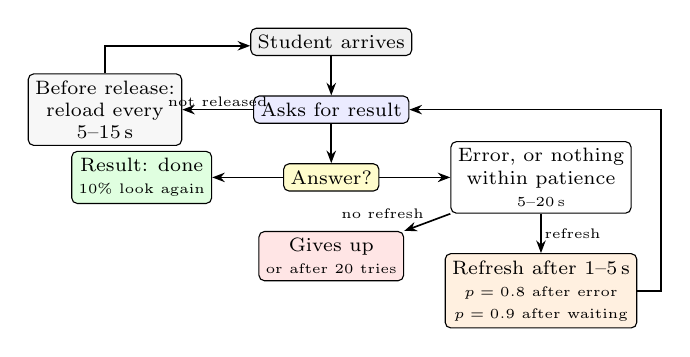
\begin{tikzpicture}[
  node distance=5mm and 6mm,
  blk/.style={draw, rounded corners=2pt, align=center, font=\scriptsize, inner sep=2.5pt, fill=white},
  dec/.style={blk, fill=yellow!20},
  arr/.style={-{Stealth[length=1.6mm]}, semithick},
  lab/.style={font=\tiny, inner sep=1pt, align=center},
]
  \node[blk, fill=gray!12] (arrive) {Student arrives};
  \node[blk, fill=blue!8, below=of arrive] (ask) {Asks for result};
  \node[blk, fill=gray!6, left=9mm of ask] (early) {Before release:\\reload every\\5--15\,s};
  \node[dec, below=of ask] (what) {Answer?};
  \node[blk, fill=green!12, left=9mm of what] (ok) {Result: done\\{\tiny 10\% look again}};
  \node[blk, right=9mm of what] (bad) {Error, or nothing\\within patience\\{\tiny 5--20\,s}};
  \node[blk, fill=orange!12, below=of bad] (refresh) {Refresh after 1--5\,s\\{\tiny $p=0.8$ after error}\\{\tiny $p=0.9$ after waiting}};
  \node[blk, fill=red!10, below=of what] (quit) {Gives up\\{\tiny or after 20 tries}};
  \draw[arr] (arrive) -- (ask);
  \draw[arr] (ask.west) -- node[lab, above] {not released} (early.east);
  \draw[arr] (early.north) |- ([yshift=-0.5mm]arrive.west);
  \draw[arr] (ask) -- (what);
  \draw[arr] (what) -- (ok);
  \draw[arr] (what) -- (bad);
  \draw[arr] (bad) -- node[lab, right] {refresh} (refresh);
  \draw[arr] (bad.south west) -- node[lab, above left] {no refresh} (quit.north east);
  \draw[arr] (refresh.east) -- ++(3mm,0) |- (ask.east);
\end{tikzpicture}

\caption{How each simulated student behaves. All numbers are assumptions;
Section~\ref{sec:rq4} varies them.}
\label{fig:student}
\end{figure}

The data are \num{200000} synthetic students with six subjects each,
generated from a seed so that the right answer for any roll number can be
recomputed; no real student data was used. Students arrive as an open-loop
Poisson process~\cite{schroeder2006open}: the rate rises over the \SI{20}{s}
before release to 20\% of the peak, reaches the peak within \SI{3}{s} of
release and decays with a time constant of \SI{30}{s} over \SI{90}{s}. Real
result days stay busy far longer~\cite{ht2021ssc}; we compress the surge to
keep runs short. Early students reload every 5--\SI{15}{s} until release. Each
student waits 5--\SI{20}{s} for an answer; after an error they refresh with
probability 0.8, after waiting in vain with probability 0.9, after a pause of
1--\SI{5}{s}, for at most 20 attempts. These numbers are assumptions;
Section~\ref{sec:rq4} varies them.

\subsection{Testbed and measurement}

All runs used one desktop computer (AMD Ryzen~7 5800X, 8 cores, \SI{32}{GB},
Windows~11 with WSL\,2 and Docker~29.9). The design under test was pinned to
the two hardware threads of one core and the load generator to twelve threads
on six other cores. We first found design A's capacity: the highest constant
arrival rate at which 99\% of students got a correct result within
\SI{2}{s}, \CapA\ students/s. Loads are multiples of it; the JEE 2016
incident was about 5$\times$~\cite{pagalguy2016jee}. An oracle classifies every
response as correct, stale (the old version after a correction), wrong,
missing (``not found'' for a real student) or failed. We report the share of
students who got a correct result within 5 or \SI{10}{s} of their first
request after release, or at all, and the CPU-seconds used by all containers
per \num{1000} students served. Each configuration ran 3 times in random
order; we report medians with 95\% bootstrap intervals. Against k6's
constant-arrival-rate executor~\cite{k6docs} at 150 requests/s, our generator
measured median latencies of 5.3--\SI{5.5}{ms} against \SI{5.4}{ms}. Six
waiting-room runs in which the generator ran out of local ports were discarded
and run again with a wider port range.

\section{Results and Discussion}
\label{sec:results}

\begin{figure*}[t]
\centering
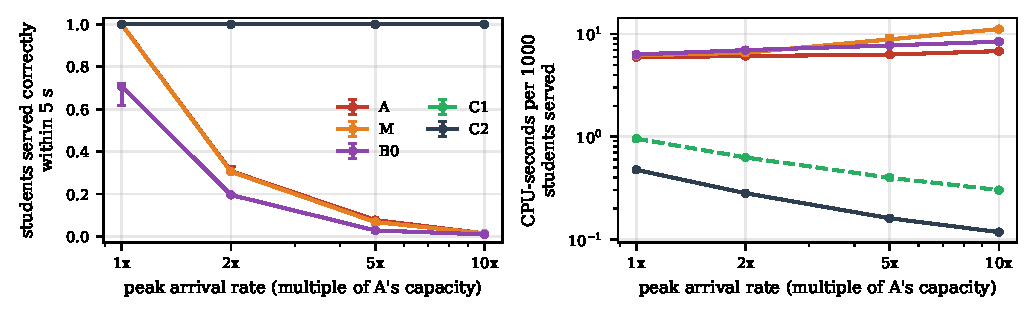
\includegraphics[width=\textwidth]{figures/core.pdf}
\caption{Q1. Left: share of students who got their correct result within
\SI{5}{s}. Right: CPU-seconds per \num{1000} students served (log scale).
Medians of 3 runs with 95\% bootstrap intervals; students do not refresh in
these runs. C1 (dashed) and C2 overlap at 100\%.}
\label{fig:core}
\end{figure*}

No run in any experiment returned a wrong result, and no container crashed.

\subsection{Q1: Which architecture?}
\label{sec:rq1}

Fig.~\ref{fig:core} compares five designs from 1$\times$ to 10$\times$ A's
capacity, with students who do not refresh so that every design faces the same
requests. A served every student within \SI{5}{s} at 1$\times$ but only
30.8\% at 2$\times$, 7.7\% at 5$\times$ and 1.4\% at 10$\times$; at
10$\times$ only 20.6\% got a result at all. Mirrors (M) matched A at 2$\times$
and did worse beyond it, using up to 1.64 times A's CPU per student. A cold
cache (B0) was worse than no cache, serving only 70.8\% within \SI{5}{s} even
at 1$\times$. The pre-computed designs C1 and C2 served every student at every
load, with 99th-percentile latencies below \SI{0.7}{ms}, and used 12.5 to 57.8
times less CPU per student than A. C1's capacity is at least \CapCOne\
students/s (33.6 times A's), where our generator ran out. Pre-computing all
\num{200000} results took 6.9--\SI{7.0}{s} (C1) and 9.4--\SI{9.8}{s} (C2).
With a page-building cost of \SI{2}{ms} or \SI{0}{ms} instead of \SI{5}{ms},
A and B0 served at least 99.8\% of students within \SI{5}{s} at the same load
as 2$\times$, so this assumption decides how much load a database-backed
portal can take. The cost order did not change: per student served, A used
2.6 (\SI{0}{ms}) to 9.7 (\SI{2}{ms}) times the CPU of C2, and B0 always used
more than A.

\subsection{Q2: Does a waiting room help?}
\label{sec:rq2}

\begin{table}[t]
\caption{Design A alone and behind a waiting room at 5$\times$ with refreshing students (median of 3 runs; run ends 135\,s after release).}
\label{tab:wr}
\centering
\footnotesize
\setlength{\tabcolsep}{2.5pt}
\begin{tabular}{@{}lrrrrr@{}}
\toprule
Waiting room & \multicolumn{2}{c}{Served (\%)} & Waiting & Wait & $\tau$ \\
\cmidrule(lr){2-3}
 & 10\,s & at all & at end (\%) & p50 (s) & \\
\midrule
none (A alone) & 6.1 & 43.3 & 0.0 & 0.2 & 0.09 \\
FIFO, token & 4.1 & 36.8 & 52.2 & 40.6 & 0.79 \\
FIFO, naive & 3.7 & 41.9 & 58.1 & 59.5 & 0.60 \\
lottery, token & 4.4 & 34.2 & 52.5 & 38.2 & 0.01 \\
lottery, naive & 3.8 & 41.8 & 58.1 & 59.8 & -0.01 \\
\bottomrule
\end{tabular}
\end{table}


Table~\ref{tab:wr} shows A alone and behind each waiting room at 5$\times$
with refreshing students. Within this \SI{135}{s} run the waiting room served
no more students than A alone (34.2--41.9\% against 43.3\%), but A's
unserved students had given up while 52--58\% of the waiting room's were
still queued. We therefore ran FIFO again with \SI{240}{s} more for the queue
to empty. It then served 98.3\% of students with naive tickets, but the
median student waited \SI{121}{s} to be admitted (95th percentile
\SI{282}{s}); in our model, queued students wait up to 10 minutes, and real
ones may leave sooner. With tokens it served only 74.5\%: admitted students
who ran out of patience refreshed straight at A, which received 3.21 requests
per student instead of 1.07. Only FIFO with tokens kept arrival order
(Kendall's $\tau=0.79$ between arrival and admission order for early
students, Table~\ref{tab:wr}); naive tickets lowered it to 0.60 because a
refresh sent the student to the back, and the lottery gave $\tau\approx0$,
like A alone. In front of C1, which needs no protection, the waiting room only added
delay and raised the CPU per \num{1000} students from 0.44 to 0.77--0.78
CPU-seconds.

\subsection{Q3: Are the results correct?}
\label{sec:rq3}

We published corrections for 1\% of students \SI{30}{s} after release at
1$\times$. Most students look once and had already looked, so corrected
students received only about 90 answers after the correction in the three
runs of each design. A, B0 with cache invalidation, and C1 gave at most one
old result, while the correction was being written (it finished within
\SI{0.19}{s}). B0 without invalidation served old results for up to
\SI{10.89}{s}, and would until its 10-minute lifetime ended; C2 served old
files from Nginx's 30-second file cache for up to \SI{13.69}{s}. When only
90\% of results were ready at release, C1 wrote the rest in \SI{0.08}{s} and
C2 in \SI{1.63}{s}, and one student was told ``not found''; a slower
preparation would leave more students without a result for longer.

\subsection{Q4: Caches and refreshing students}
\label{sec:rq4}

At 2$\times$, with every student asking for a different roll number, every
cache miss in B0 was the first request for that key; no two requests ever
raced for the same key. Request coalescing (B1) and early recomputation (B2)
therefore changed nothing (8.5--8.9\% served within \SI{5}{s}), while filling
the cache before release (B3) served everyone, at 0.71 CPU-seconds per
\num{1000} students against B0's 6.27.

\begin{figure*}[t]
\centering
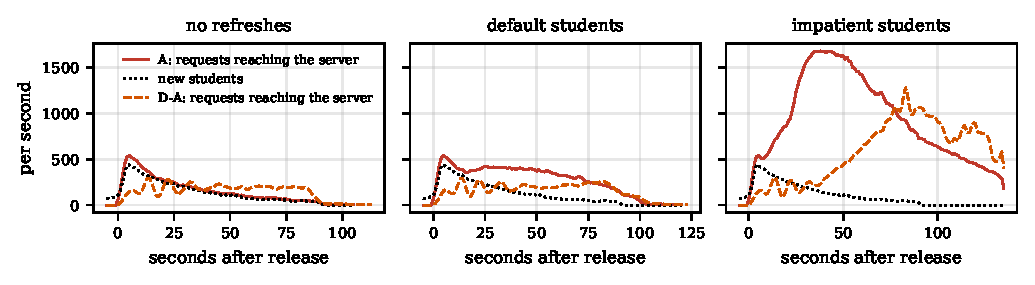
\includegraphics[width=\textwidth]{figures/refresh.pdf}
\caption{Q4. Requests reaching the server each second for A alone (solid) and
behind a waiting room (D-A, dashed) at 2$\times$, against new students
(dotted). One run per kind of student.}
\label{fig:refresh}
\end{figure*}

Refreshing changes the load a lot (Fig.~\ref{fig:refresh}). For A at
2$\times$, students who never
refresh sent 1.17 requests each; our default students sent 2.23, so more were
served in the end (88.1\% against 77.7\%) but fewer within \SI{10}{s} (32.7\%
against 53.7\%). Impatient students (patience 3--\SI{8}{s}) sent 8.65 requests
each and kept A overloaded until the end of every run; only 22.1\% were
served. Behind a waiting room the load on A stayed near one request per
student with default students (1.32), but with impatient students A still
received 5.30 requests per student.

\subsection{Decision guide}

\begin{table}[t]
\caption{Decision guide for examination boards, from our measurements}
\label{tab:guide}
\centering
\footnotesize
\setlength{\tabcolsep}{3pt}
\begin{tabular}{@{}>{\raggedright\arraybackslash}p{2.5cm}>{\raggedright\arraybackslash}p{3.1cm}>{\raggedright\arraybackslash}p{2.3cm}@{}}
\toprule
If the board\ldots & then\ldots & because (section)\\
\midrule
has the results before release & publishes them pre-computed, as files or in a key--value store & served 10$\times$ at 12.5--57.8$\times$ less CPU (\ref{sec:rq1})\\
must build pages from a database & does not count on mirrors or an empty cache; fills the cache before release & M and B0 no better than A; B3 served all (\ref{sec:rq1}, \ref{sec:rq4})\\
cannot finish preparing by release time & delays the release & early students are told ``not found'' (\ref{sec:rq3})\\
corrects results after release & deletes or rewrites every cached copy and keeps file caches short & old results for up to \SI{14}{s} otherwise (\ref{sec:rq3})\\
expects students to refresh & makes the page retry by itself, with back-off & impatient students kept A down (\ref{sec:rq4})\\
considers a waiting room in front of a slow website & uses one only if students can wait minutes; admits FIFO; does not let admitted students refresh without limit & served 98.3\% instead of 43.3\%, after a \SI{121}{s} median wait; 74.5\% with tokens (\ref{sec:rq2})\\
\bottomrule
\end{tabular}
\end{table}

Table~\ref{tab:guide} turns these results into advice. The numbers come from
one machine and should be read as relative, not absolute.

\textbf{Limitations.} All runs used one machine, no content delivery network
and a surge compressed to \SI{90}{s}. The students and the page-building cost
are models. Three runs per configuration give wide intervals for some
measures. We have not yet measured a real result day.

\section{Conclusion}

With ResultBench we measured eleven designs of a result website under the same
budget. Building pages on request failed by twice the capacity of a
database-backed portal, while pre-computed results served ten times that load
at a small fraction of the CPU. Wrong results never appeared, and old results
lasted more than a moment only where cached copies were not updated. Stampede defences do not
help when every student asks for a different result, and refreshing students
can keep a portal overloaded. A waiting room in front of an overloaded portal
served almost everyone, but only after waits of minutes, and fewer when
admitted students could keep refreshing. Next, we plan to measure real result days and to test
real portal software and multi-server deployments. ResultBench is open source
(MIT licence) at \url{https://github.com/K144U/NoCrashing}.

\section*{Acknowledgments}

An AI assistant (Claude Opus 5.5, Anthropic) was used under the authors'
direction for software development, data analysis, figures, and drafting and
editing of the text. The authors reviewed all content and are responsible for
it.


\bibliographystyle{IEEEtran}
\bibliography{refs}

\end{document}
